\documentclass[letterpaper,11pt]{article}
\usepackage{etex}
\reserveinserts{28}
\usepackage{amssymb}
\usepackage{theorem}
%\usepackage{savetrees}
\usepackage[margin=2cm]{geometry}
\usepackage{graphicx}
\usepackage{fancybox}
\usepackage{fancyhdr}
\usepackage{tabularx}
\usepackage{color}
\usepackage{xcolor}
\usepackage{multirow}
\usepackage{amsmath}
\usepackage[utf8]{inputenc} % Pour pouvoir taper les accent directement et non pas passer par \'
\usepackage[T1]{fontenc} %%% Pour que les accents soient correctement traités dans le PDF et le DVI
\usepackage{lmodern} %Un autre package pour les accents français
\usepackage[french]{babel} %Un autre package pour les accents
\usepackage{ifthen}
%\usepackage{multicol}
%\usepackage{cancel}
\usepackage{pst-all}
\usepackage{pstricks-add}
\usepackage{multicol}
%\usepackage{tikz}
%\usepackage{pgf,tikz}
%\usepackage{circuitikz}
%\usetikzlibrary{shapes}
%\usetikzlibrary{calc}
%\usetikzlibrary{plotmarks}
%\usepackage{tkz-fct}
\usepackage{fp}
\usepackage{float}
\usepackage{siunitx}
\usepackage{pdfpages}%Pour sortir seulement certaine pages du pdf
\usepackage{textcomp}
\usepackage{hyperref}
\hypersetup{
    colorlinks=true, % make the links colored
    linkcolor=blue, % color TOC links in blue
    urlcolor=red, % color URLs in red
    linktoc=all % 'all' will create links for everything in the TOC
}

\sisetup{locale = FR, number-math-rm, per-mode=symbol, separate-uncertainty}

\renewcommand{\exp}[1]{\mathrm{e}^{#1}}

\setlength{\parindent}{0pt}



\begin{document}


\begin{center}
~
\vfill
\LARGE{Travail Pratique 2 (IFT-4201/IFT-7201)}\\[0.4cm]

\Large{Présenté à Audrey Durand}

\vfill
\large{Équipe 10: Adam Cohen, Maxime Genest, Vincent Masse}

\vfill
\thispagestyle{empty}

\end{center}

\clearpage

\pagestyle{fancy}
\lhead{IFT-7201}
\chead{Devoir 2 (Automne 2020)}
\rhead{Équipe 10}


\begin{enumerate}

\item

\begin{enumerate}

\item 

\item \textbf{Réseau cible}\\
L'oubli catastrophique est le fait qu'un réseau de neurones oubli son apprentissage lorsqu'il doit apprendre une nouvelle tâche, c'est un peu comme s'il recommençait son apprentissage à 0. Le fait de fixer les poids $\theta$ dans la cible pendant plusieurs mise à jours permet de conserver une certaine stabilité pour permettre la convergence.

\item \textbf{Heuristique}\\
Si $\tau$ est trop grand, la cible est trop modifié, ce qui risque de compromettre la convergence (voir numéro précédent), le cas limite $\tau=1$ revient à ne pas fixer (même pas partiellement) les targets. Si $\tau$ est trop petit, les targets seront trop fixes, et donc les cibles ne sont pratiquement pas améliorées et le réseau apprend donc sur des moins bonnes cibles (non-représentative de ce que l'on doit viser). Le cas limite $\tau=0$ montre un cas où la cible n'est jamais modifiée et gardera toujours sa valeur initiale, ce qui est bien entendu non-souhaitable. 

\item \textbf{Replay buffer}\\
L'avantage de son utilisation est de briser la corrélation entre les échantillons utilisés lors de la mise à jour (le tuple $(s_t, a_t, r_{t+1}, s_{t+1})$ et le tuple suivant $(s_{t+1}, a_{t+1}, r_{t+2}, s_{t+2})$ partage le même état $s_{t+1}$). Cela compromet l'apprentissage. Le fait de stocker les échantillons et d'échantillonner une mini-batch plusieurs fois au cours de l'épisode permet contourner ce problème. À COMPLÉTER  

\item \text{Apprentissage supervisée}\\


\item Graphiques...

\begin{center}
\begin{figure}[H]
\caption{Évolution des gains et fonction de pertes}
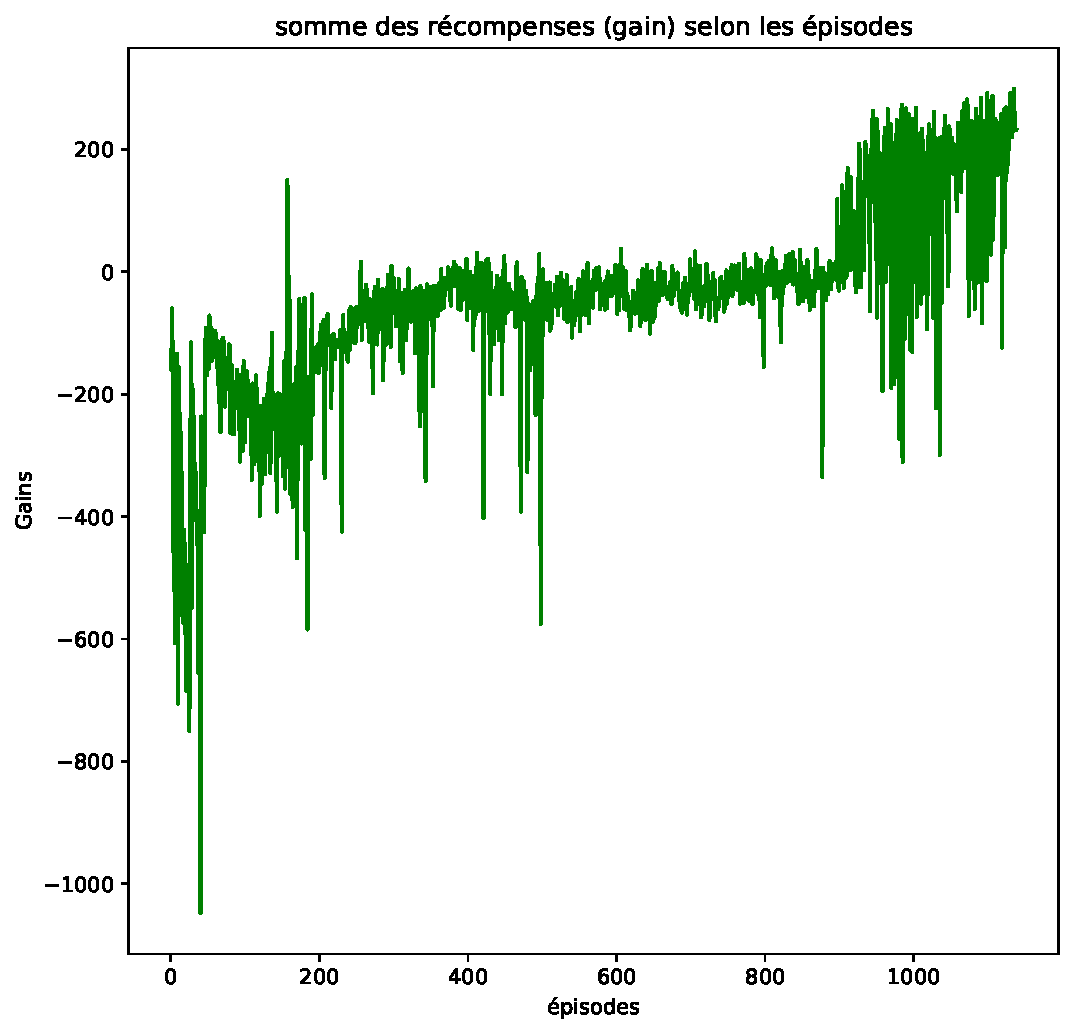
\includegraphics[width=0.45\linewidth]{gains.pdf} \hfill 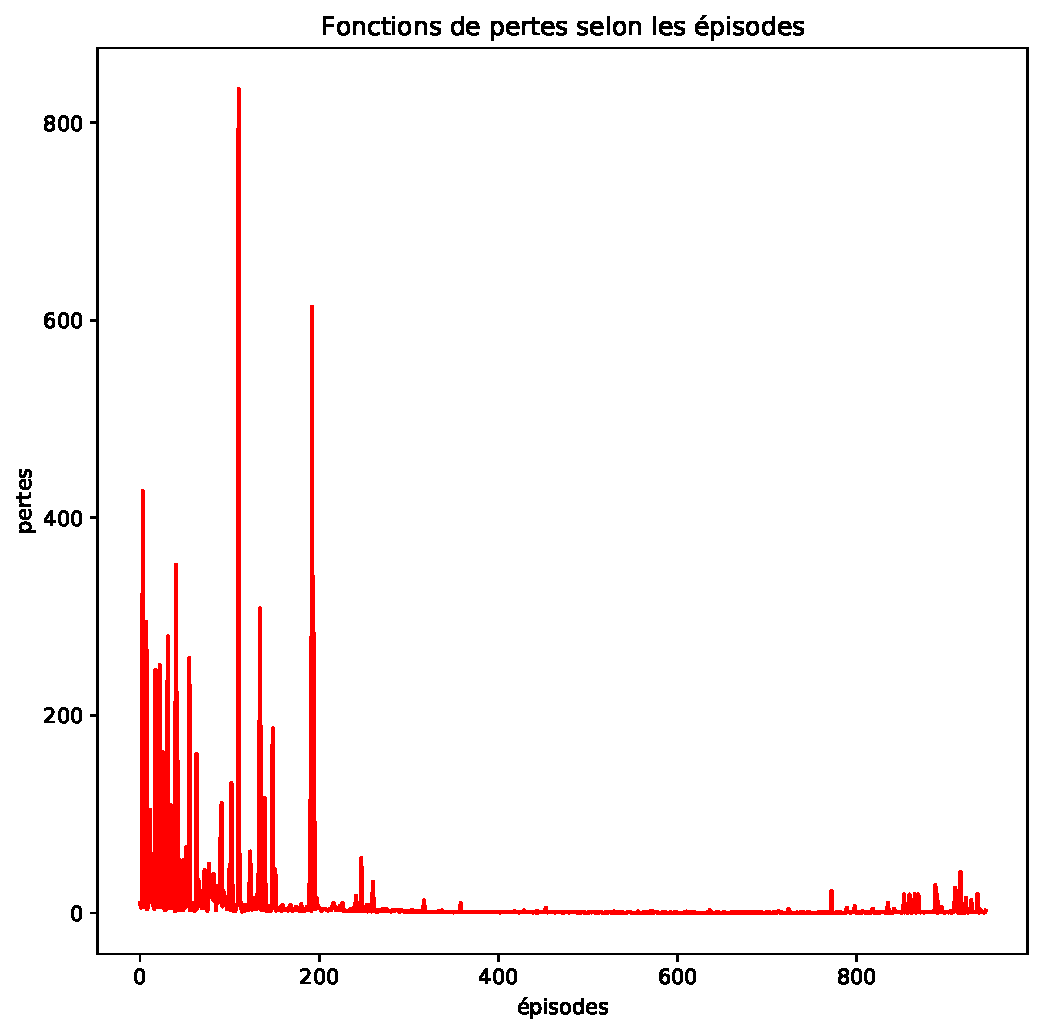
\includegraphics[width=0.45\linewidth]{pertes.pdf}
\end{figure}
\end{center}

FONCTION DE PERTE CI-DESSUS À MODIFIER (Je ne suis pas certain que c'est ça qu'il est demandé)


\begin{figure}[H]
\begin{center}
\caption{}
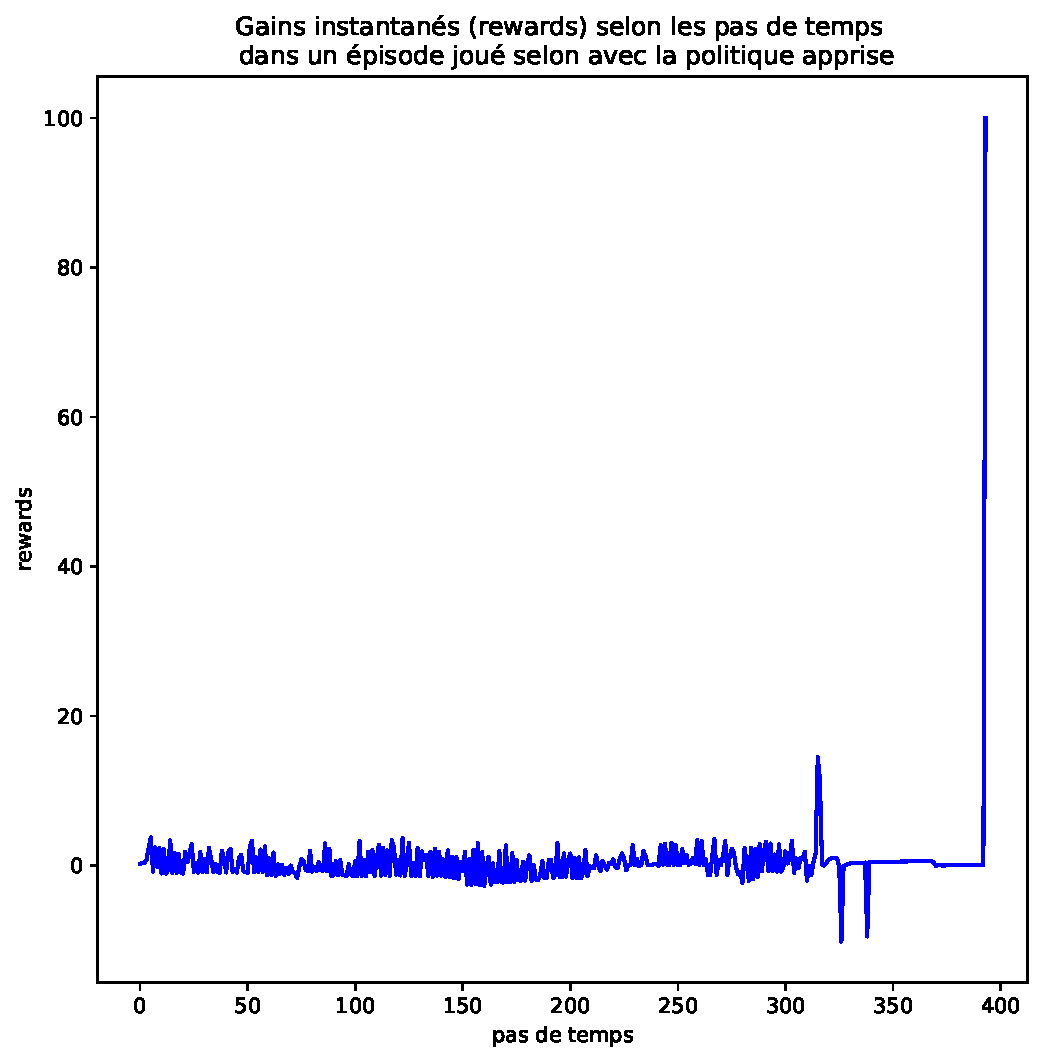
\includegraphics[scale=0.5]{gain_par_pas.pdf}
\end{center}
\end{figure}

\end{enumerate}

\item No 2

\begin{enumerate}

\item

\item

\end{enumerate}

\end{enumerate}

\end{document}
